% ============================================================
%  Příprava na maturitu – Elektrotechnika
%  Okruh 11: Pasivní elektronické součástky
% ============================================================

\documentclass[a4paper,10pt]{article}

\usepackage[T1]{fontenc}
\usepackage[utf8]{inputenc}
\usepackage[left=2.0cm, right=1.8cm, top=1.8cm, bottom=1.8cm]{geometry}
\usepackage{parskip}
\usepackage{xcolor}
\usepackage{tabularx}
\usepackage{booktabs}
\usepackage{tikz}
\usepackage{mdframed}
\usepackage{amsmath}
\usepackage{enumitem}
\usepackage{circuitikz}

\usetikzlibrary{arrows.meta, positioning, decorations.pathmorphing, shapes.geometric, calc}

% --- Barvy ---
\definecolor{accent}{HTML}{1A3A5C}
\definecolor{lightblue}{HTML}{EAF2F8}
\definecolor{lightyellow}{HTML}{FDFBE4}
\definecolor{lightgreen}{HTML}{EAF7EA}
\definecolor{lightred}{HTML}{FDE8E8}
\definecolor{lightgray}{HTML}{F4F4F4}

% --- Boxy ---
\newmdenv[backgroundcolor=lightblue,linecolor=accent!40,roundcorner=4pt,
  innertopmargin=6pt,innerbottommargin=6pt,innerleftmargin=8pt,innerrightmargin=8pt]{pojmybox}
\newmdenv[backgroundcolor=lightyellow,linecolor=accent!30,roundcorner=4pt,
  innertopmargin=6pt,innerbottommargin=6pt,innerleftmargin=8pt,innerrightmargin=8pt]{vysvetlenibox}
\newmdenv[backgroundcolor=lightgreen,linecolor=accent!40,roundcorner=4pt,
  innertopmargin=6pt,innerbottommargin=6pt,innerleftmargin=8pt,innerrightmargin=8pt]{vzorcebox}
\newmdenv[backgroundcolor=lightred,linecolor=accent!30,roundcorner=4pt,
  innertopmargin=6pt,innerbottommargin=6pt,innerleftmargin=8pt,innerrightmargin=8pt]{durazbox}

\setlist[itemize]{noitemsep, leftmargin=1.4em, topsep=2pt}
\setlist[enumerate]{noitemsep, leftmargin=1.4em, topsep=2pt}

% --- Zkratka pro jednotky ---
\newcommand{\jednotka}[1]{\,[\mathrm{#1}]}

\begin{document}

% ============================================================
\section*{\large Okruh 11 – Pasivní elektronické součástky}

\begin{pojmybox}
\textbf{Klíčové pojmy:}
pasivní vs. aktivní součástka, rezistor, potenciometr, termistor (NTC/PTC), varistor (VDR), fotorezistor (LDR), barevný kód, kondenzátor, keramický a elektrolytický kondenzátor, cívka, RC články (filtry), SMD montáž
\end{pojmybox}

\begin{vysvetlenibox}

% ================================================================
\subsection*{1. Pasivní vs. Aktivní součástky}

\begin{itemize}
    \item \textbf{Pasivní:} Nedokážou signál zesilovat. Energii pouze spotřebovávají (mění na teplo) nebo ji dočasně akumulují v elektrickém či magnetickém poli. (Rezistory, kondenzátory, cívky).
    \item \textbf{Aktivní:} Dokážou elektrický signál zesilovat nebo aktivně spínat, potřebují k tomu napájení. (Tranzistory, diody, integrované obvody – \textit{viz Okruh 12}).
\end{itemize}

% ================================================================
\subsection*{2. Rezistory}

Rezistor je součástka, která klade průchodu proudu elektrický odpor. Její hlavní funkcí je \textbf{omezení proudu} v obvodu nebo vytvoření \textbf{děliče napětí}.

\textbf{Dělení podle provedení:}
\begin{itemize}
    \item \textbf{Pevné rezistory:} Odpor je dán z výroby (uhlíkové, metalizované, drátové pro velké výkony). Značení se provádí pomocí \textbf{barevných proužků} nebo SMD kódem.
    \item \textbf{Proměnné rezistory:} Odpor lze měnit mechanicky.
    \begin{itemize}
        \item \textbf{Potenciometr:} Má hřídelku, slouží k časté regulaci uživatelem (např. hlasitost).
        \item \textbf{Trimr:} Ovládá se šroubovákem, slouží k jednorázovému nastavení obvodu technikem ve výrobě.
    \end{itemize}
\end{itemize}

\begin{center}
\begin{circuitikz}[font=\small, thick]
  \draw (0,0) to[R, l=Rezistor] (2,0);
  \draw (3,0) to[pR, l=Potenciometr] (5,0);
  \draw (7.5,0.7) node[circle, draw, inner sep=1pt] {A} -- (7.5,0) to[R, l=Dělič napětí] (7.5,-2) node[circle, draw, inner sep=1pt] {B};
  \draw (7.5, -0.8) to[short, *-o] (9, -0.8) node[right] {$U_{out}$};
\end{circuitikz}
\end{center}

% ================================================================
\subsection*{3. Nelineární rezistory}

Jejich odpor se nemění mechanicky, ale v závislosti na nějaké fyzikální veličině.

\begin{center}
\begin{tabularx}{0.97\linewidth}{@{} l X @{}}
\toprule
\textbf{Typ součástky} & \textbf{Vlastnost a použití} \\
\midrule
\textbf{Termistor NTC} & \textit{Negative Temperature Coefficient.} S rostoucí teplotou odpor \textbf{klesá}. Použití: Měření teploty (teploměry). \\
\textbf{Termistor PTC} & \textit{Positive Temperature Coefficient.} S rostoucí teplotou odpor \textbf{roste}. Použití: Ochrana proti přehřátí, PTC topná tělíska. \\
\textbf{Varistor (VDR)} & \textit{Voltage Dependent Resistor.} Při překročení určitého napětí odpor prudce \textbf{klesne} a zkratuje obvod. Použití: Ochrana proti přepětí (\textit{viz Okruh 10}). \\
\textbf{Fotorezistor (LDR)}& \textit{Light Dependent Resistor.} S rostoucím osvětlením odpor \textbf{klesá}. Použití: Soumrakové spínače. \\
\bottomrule
\end{tabularx}
\end{center}

\begin{center}
\begin{circuitikz}[font=\small, thick]
  \draw (0,0) to[thR, l=Termistor] (2,0);
  \draw (3,0) to[vR, l=Varistor] (5,0);
  \draw (6,0) to[phR, l=Fotorezistor] (8,0);
\end{circuitikz}
\end{center}

% ================================================================
\subsection*{4. Kondenzátory}

Akumulují elektrický náboj v elektrostatickém poli (\textit{viz Okruh 2}). V obvodech \textbf{stejnosměrného proudu (DC)} se po nabití chovají jako \textbf{rozpojený obvod}. V obvodech \textbf{střídavého proudu (AC)} jimi prochází proud (klade \textbf{kapacitní reaktanci $X_C$}, viz Okruh 4).

\textbf{Hlavní typy:}
\begin{itemize}
    \item \textbf{Keramické a fóliové:} Malé kapacity (pF až nF). Nejsou polarizované (lze je zapojit libovolně). Výborné pro vysoké frekvence (filtrace rušení).
    \item \textbf{Elektrolytické:} Velké kapacity ($\mu$F až mF). Dosahují toho navinutím hliníkových fólií s elektrolytem. \textbf{Jsou polarizované (+ a $-$)}.
\end{itemize}

\begin{durazbox}
\textbf{Kritické varování:} Elektrolytický kondenzátor se musí zapojit správnou polaritou. Při přepólování dojde uvnitř k chemické reakci, vývinu plynu a **explozi součástky**!
\end{durazbox}

\begin{center}
\begin{circuitikz}[font=\small, thick]
  \draw (0,0) to[C, l=Běžný] (2,0);
  \draw (3,0) to[eC, l=Elektrolyt] (5,0);
  \node[above, red] at (3.5, 0.3) {$+$};
  \draw (6,0) to[vC, l=Ladicí] (8,0);
\end{circuitikz}
\end{center}

% ================================================================
\subsection*{5. Cívky (Induktory)}

Akumulují energii do magnetického pole (\textit{viz Okruh 3}). Chovají se opačně než kondenzátory: \textbf{stejnosměrný proud (DC)} propouštějí s minimálním odporem, ale \textbf{střídavému proudu (AC)} kladou odpor (\textbf{induktivní reaktance $X_L$}, viz Okruh 4) a brání rychlým změnám proudu.

\begin{itemize}
    \item \textbf{Vzduchové cívky:} Mají malou indukčnost, používají se pro vysoké frekvence (vysílače, rádia).
    \item \textbf{Cívky s feritovým jádrem:} Ferit (magneticky měkký materiál) výrazně zvyšuje indukčnost. Slouží často jako \textbf{tlumivky} – tlumí vysokofrekvenční rušení ve zdrojích.
\end{itemize}

% ================================================================
\subsection*{6. Využití součástek: RC filtry}

Kombinací rezistoru a kondenzátoru tvoříme frekvenční filtry. Využívá se faktu, že odpor kondenzátoru (reaktance) pro vysoké frekvence klesá.

\begin{center}
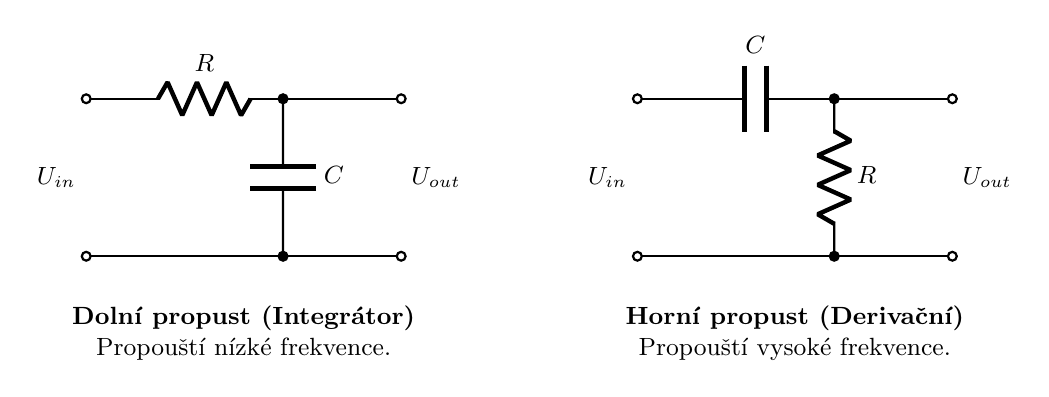
\begin{tikzpicture}[>=Stealth, font=\small, thick]
  % Dolní propust
  \begin{scope}[xshift=0cm]
    \draw (0,2) to[short, o-] (0.5,2) to[R, l=$R$] (2.5,2) to[short, -o] (4,2);
    \draw (0,0) to[short, o-o] (4,0);
    \draw (2.5,2) to[C, l=$C$, *-*] (2.5,0);
    \node[left] at (0,1) {$U_{in}$};
    \node[right] at (4,1) {$U_{out}$};
    \node[align=center, below=0.5cm] at (2,0) {\textbf{Dolní propust (Integrátor)}\\Propouští nízké frekvence.};
  \end{scope}

  % Horní propust
  \begin{scope}[xshift=7cm]
    \draw (0,2) to[short, o-] (0.5,2) to[C, l=$C$] (2.5,2) to[short, -o] (4,2);
    \draw (0,0) to[short, o-o] (4,0);
    \draw (2.5,2) to[R, l=$R$, *-*] (2.5,0);
    \node[left] at (0,1) {$U_{in}$};
    \node[right] at (4,1) {$U_{out}$};
    \node[align=center, below=0.5cm] at (2,0) {\textbf{Horní propust (Derivační)}\\Propouští vysoké frekvence.};
  \end{scope}
\end{tikzpicture}
\end{center}

% ================================================================
\subsection*{7. Technologie montáže (THT vs. SMD)}

\begin{itemize}
    \item \textbf{THT (Through-Hole Technology):} Klasické součástky s drátovými vývody. Zasouvají se do děr v desce plošných spojů (DPS) a pájí z druhé strany.
    \item \textbf{SMD (Surface Mount Devices):} Součástky pro \textbf{povrchovou montáž}. Nemají drátky, jen malé plošky. Pájí se přímo na povrch desky. Umožňují obrovskou miniaturizaci a automatickou výrobu stroji. Kódy na SMD rezistorech: $103 = 10 \cdot 10^3\,\Omega = 10\,\mathrm{k\Omega}$.
\end{itemize}

% ================================================================
\subsection*{8. Shrnutí – Přehled chování v obvodu}

\begin{center}
\begin{tabularx}{0.97\linewidth}{@{} l X X @{}}
\toprule
\textbf{Součástka} & \textbf{Na stejnosměrném (DC)} & \textbf{Na střídavém (AC)} \\
\midrule
\textbf{Rezistor ($R$)} & Omezuje proud ($I = U/R$) & Omezuje proud (beze změny fáze) \\
\textbf{Kondenzátor ($C$)} & Nabije se a proud obvodem neteče & Propouští proud, zpožďuje napětí \\
\textbf{Cívka ($L$)} & Propouští (jen odpor drátu) & Klade odpor, zpožďuje proud \\
\bottomrule
\end{tabularx}
\end{center}

\end{vysvetlenibox}

\end{document}